\subsection{Extrapolate velocities}

Sometimes it happens that some of the edges on the grid are close to the surface but no particle was close enough to update the velocity of the edge. We still want this edges to be part of our pressure solve on the grid. This will make it easier to setup the pressure equations later on. This means we have to guarantee that we have valid velocities on the grid where the level set tells us an edge or cell is inside or close to the surface of the fluid. To ensure this, we will extrapolate the velocities from the surface and outwards with the help of the level set. Remember from section 2.3 that the gradient of the level set is the same as the normal of the surface. If we extrapolate the velocities in the direction of the normal, the derivate of the velocities along the normal should be zero. Figure \ref{extrapic} shows an example of extrapolating the velocities along the normal.

\begin{figure}[ht!]
\centering
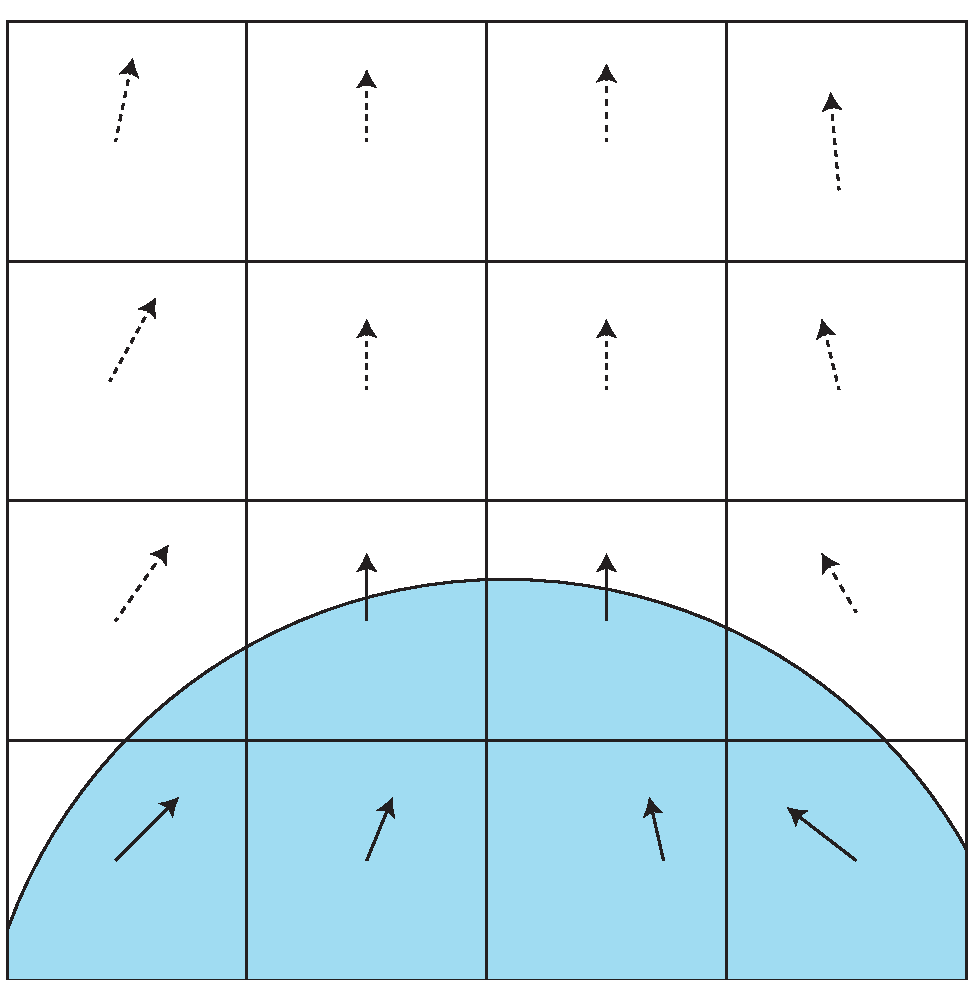
\includegraphics[width=60mm]{img/extrapolate.pdf}
\caption{The velocities of the cells inside the fluid (marked as solid arrows) are extrapolated in the surface normal direction (marked as dashed arrows).}
\label{extrapic}
\end{figure}

We can use this condition to have create an iterative solution to the unknown velocities outside of the surface. The following equations say that the horizontal velocity $u$ should be constant along the normal of the surface.

\begin{equation}
\begin{split}
\nabla \phi \cdot \nabla u &= 0 \\
\frac{\partial \phi}{\partial x}\frac{\partial u}{\partial x} + 
\frac{\partial \phi}{\partial y}\frac{\partial u}{\partial y}&= 0
\end{split}
\label{extrapolate}
\end{equation}

To find an expression that we can solve iteratively we need to approximate the partial derivates similar to what we did in previous section. Then we use the fast sweeping method once more. Notice that Equation \ref{extrapolate} is only for the horizontal velocities $u$ and one has to solve vertical velocities $v$ indiviually. It is important that the fast sweeping algorithm only updates velocities on edges that did not recieve any velocities from the particles because we do not want the velocity field to be constant in the negative direction of the normal.
